\documentclass[a4paper]{article}

\usepackage{pgfplots}

\pgfplotsset{compat=1.7}

\begin{document}

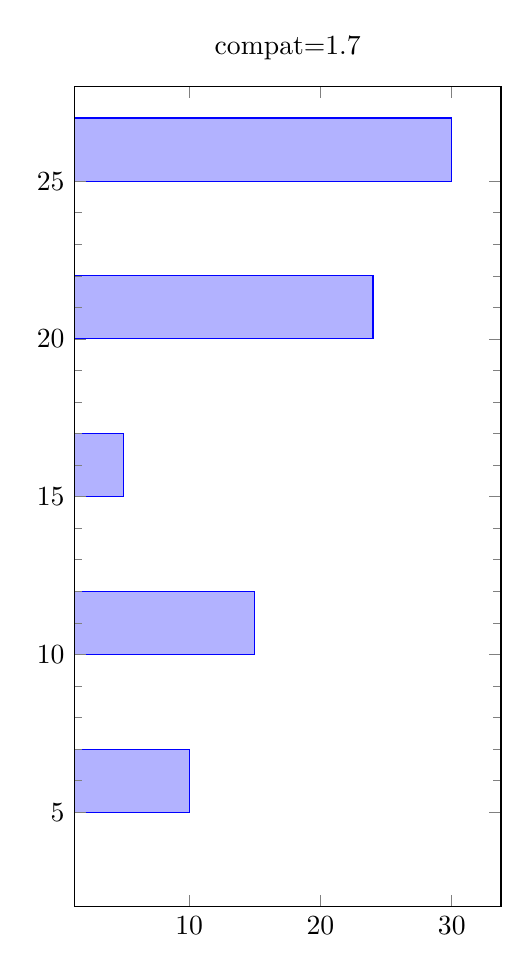
\begin{tikzpicture}
\begin{axis}[
	title={compat=1.7},
	/tikz/xbar,
	width=7cm,
	height=12cm,
	bar width=2,
	bar shift=1,
	minor y tick num=4,
	ytick=data,
	area style,
	enlargelimits=0.15]
\addplot
coordinates
    {(10,5) (15,10) (5,15) (24,20) (30,25)};
\end{axis}
\end{tikzpicture}
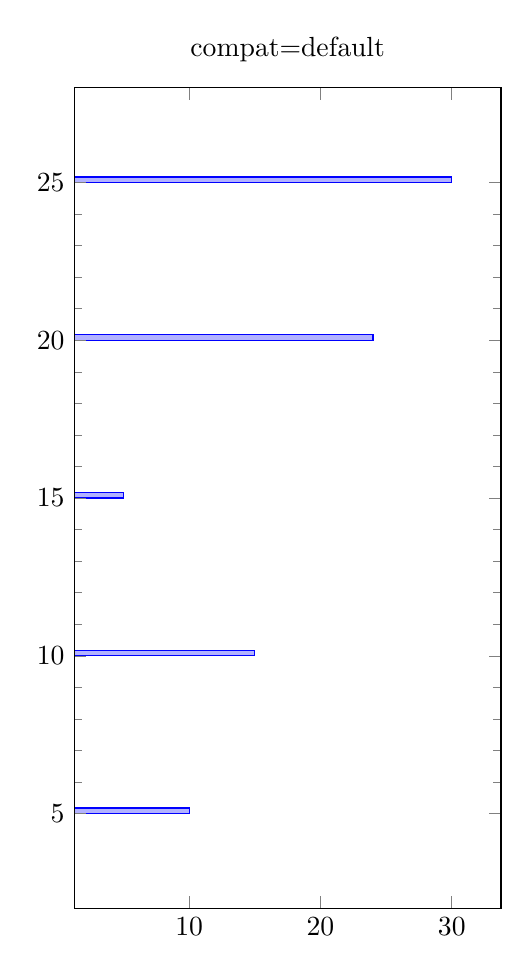
\begin{tikzpicture}
\pgfplotsset{compat=default}
\begin{axis}[
	title={compat=default},
	/tikz/xbar,
	width=7cm,
	height=12cm,
	bar width=2,
	bar shift=1,
	minor y tick num=4,
	ytick=data,
	area style,
	enlargelimits=0.15]
\addplot
coordinates
    {(10,5) (15,10) (5,15) (24,20) (30,25)};
\end{axis}
\end{tikzpicture}

\end{document}

